\begin{figure}[H]
\begin{center}
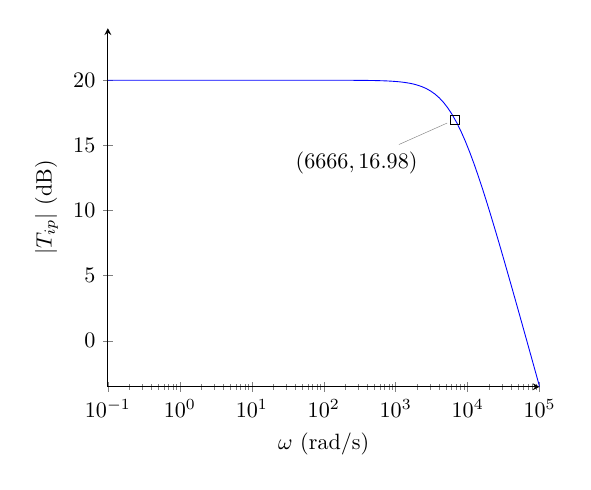
\begin{tikzpicture} [scale=0.8]
\begin{semilogxaxis}[
    axis lines = left,
    xlabel = {$\omega$ (rad/s)},
    ylabel = {$|T_{ip}|$ (dB)},
]
\addplot [
    domain=0.1:10000, 
    samples=100, 
    color=white,
]
{24*log10(10/sqrt(1+(x/6666)^2))};
\addplot [
    domain=0.1:100000, 
    samples=100, 
    color=blue,
]
{20*log10(10/sqrt(1+(x/6666)^2))};
\addplot[mark=square] coordinates {(6666,16.98)} node[pin=220:{$(6666,16.98)$}]{};
\end{semilogxaxis}
\end{tikzpicture}
\hspace{1cm}
\begin{tikzpicture} [scale=0.8]
\begin{semilogxaxis}[
    axis lines = left,
    xlabel = {$\omega$ (rad/s)},
    ylabel = {$\angle T_{ip} $ (°)},
    xtick={10,100,1000,10000,100000,1000000,10000000},
    ytick={180, 135, 90, 0},
]
\addplot [
    domain=10:10000000, 
    samples=100, 
    color=blue
]
{180-atan(x/(6666))};
\addplot[mark=square] coordinates {(6666,135)} node[pin=220:{$(6666,135)$}]{};
\addplot [
    domain=10:10000000, 
    samples=100, 
    color=white
]
{180};
\addplot [
    domain=10:10000000, 
    samples=100, 
    color=white
]
{90};
\end{semilogxaxis}
\end{tikzpicture}
\end{center}
\caption{Curvas de bode teóricas da função de transferência do integrador.}
\label{bode:1} 
\end{figure}